\documentclass[../../main.tex]{subfiles}
\begin{document}


\begin{problem}
求下面的 0 - 1 背包问题:

\begin{itemize}
    \item $N = 5$,$M = 12$,$(p_1, p_2, \dots, p_5)= (10, 15, 6, 8, 4),(w_1, w_2, \dots, w_5)=(4,6,3,4,2)$
    \item $N = 5$,$M = 15$,$(w_1, w_2, \dots, w_5) = (p_1, p_2, \dots, p_5)=(4,4,5,8,9)$
\end{itemize}
\end{problem}

\begin{solution}
\end{solution}

\begin{center}
    \begin{tikzpicture}
        \tikzset{every tree node/.style={ draw, rectangle}}
        \Tree
        [.w,p ]
    \end{tikzpicture}
\end{center}
\begin{enumerate}
    \item [1.] 已经按照$p_i / w_i$排序
\end{enumerate}
\begin{center}
    \begin{tikzpicture}
        \tikzset{every tree node/.style={ draw, rectangle}}
        \Tree
        [.0,0
        [.4,10 [.10,25 [.$w=13$ ][.10,25 [.${w}=14$ ][.10,25 [.12,29 ][.10,25 ]]]] [.4,10 [.7,16 [.$max\{p\}<28$ ]][.4,10 [.$max\{p\}<22$ ]]]]
        [.0,0 [.6,15 [.9,21 [.$max\{p\}<28.5$ ]][.6,15 [.$max\{p\}=27$ ]] ][.0,0 [.$max\{p\}<9$ ]]]
        ]
    \end{tikzpicture}
\end{center}
因此选择$(1,1,0,0,1)$,背包最大价值为29
\begin{enumerate}
    \item [2.]  $p_i / w_i$均相同
\end{enumerate}
\begin{center}
    \begin{tikzpicture}
        \tikzset{every tree node/.style={ draw, rectangle}}
        \Tree
        [.0,0
        [.4,4
        [.8,8 [.13,13 [.$w=21$ ]][.$max\{p\}=8$ ]]
        [.4,4 [.9,9 [.$w=17$ ][.9,9 [.$w=18$ ][.9,9 ]]][.4,4 [.12,12 [.$w=21$ ][.12,12 ]][.4,4 [.13,13 ][.4,4 ]]]]
        ]
        [.0,0
        [.4,4 [.$max\{p\}=13$ ]]
        [.0,0 [.5,5 [.13,13 [.$max\{p\}=13$ ]][.5,5 [.14,14 ][.5,5 ]]][.$max\{p\}=9$ ]]
        ]
        ]
    \end{tikzpicture}
\end{center}
因此选择$(0,0,1,0,1)$,背包最大价值为14
\end{document}